%-------------------------------------------------------------------------------
% seq66 windows
%-------------------------------------------------------------------------------
%
% \file        seq66 windows.tex
% \library     Documents
% \author      Chris Ahlstrom
% \date        2021-02-13
% \update      2021-06-09
% \version     $Revision$
% \license     $XPC_GPL_LICENSE$
%
%     Provides a discussion of starting up Seq66 in Windows.
%
%-------------------------------------------------------------------------------

\section{Seq66 In Windows}
\label{sec:windows}

   This section discusses installing and using the basics of \textsl{Seq66}
   in \textsl{Microsoft Windows}.  Additional trouble-shooting information can be
   found in the installed file:

   \begin{verbatim}
      C:/Program Files (x86)/Seq66/data/readme.windows
   \end{verbatim}

   First, apart from cloning \textsl{Sequencer64-packages} (where the
   \textsl{Seq66} installers are kept, which is a lot
   of data), there are tricks to getting the installer
   (\texttt{seq66\_setup\_0.93.0.exe}) properly. 
   One can't just right-click and save the link.
   The file downloaded that way is broken.
   Instead, click on the link.  Then look for a "Download" button, and
   click that instead.

   Installation itself is straightforward.  Run the installer (e.g.
   \texttt{seq66\_setup\_0.93.0.exe}).  Accept the license terms (\textsl{GNU
   GPL 2 or 3}), make sure all components are selected, accept the default
   install directory, and click through until the installation is done.

   (Note that there is also a
   \texttt{qpseq66-release-package-0.93.0.7z} portable installer
   than can be download, again using the \textsl{GitHub} "Download" button.
   Just extract that file where desired.)

   Note that, although the \textsl{Windows} version can be built as a 64-bit
   application, it is currently built as a 32-bit application.

   Now run 
   \texttt{C:/Program Files (x86)/Seq66/qpseq66.exe}.
   (One might want to create a desktop short cut; one can also go to the
   "Start" menu and search for "qpseq66.exe".)
   Assuming there are no MIDI devices attached, and no other MIDI programs
   running, an error like the following will appear:

\begin{figure}[H]
   \centering 
   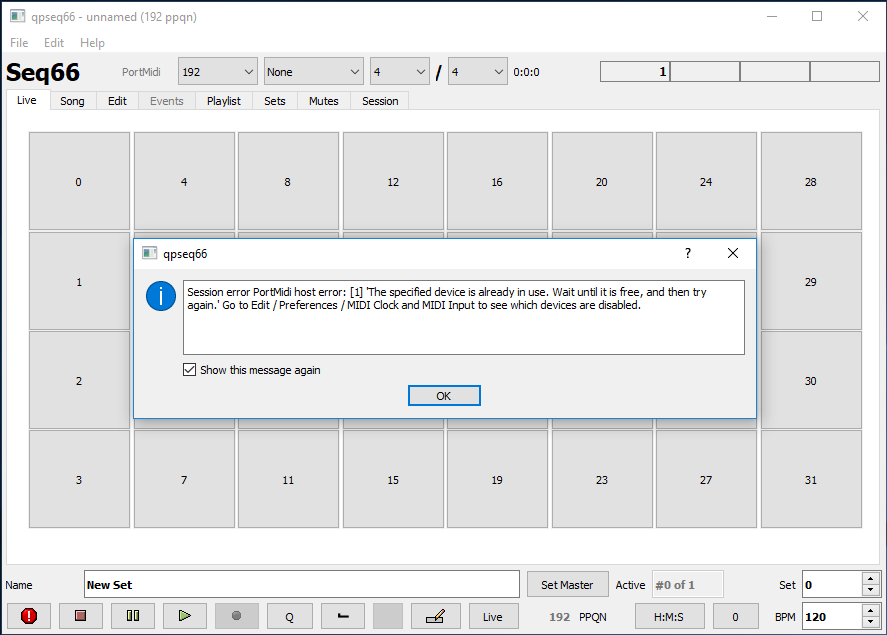
\includegraphics[scale=0.65]{windows/windows-first-startup.png}
   \caption{Seq66 First Startup in Windows}
   \label{fig:windows_first_startup}
\end{figure}

   This error occurs on \textsl{Windows 10} because the 0th port, the
   \textsl{Microsoft MIDI Mapper}, grabs access to the 1st port, the
   \textsl{Microsoft GS Wavetable Synth}.  It is fixed easily by exiting
   and rerunning the application:
   Click \textbf{OK} on the error and then \textbf{File / Quit}.
   \textsl{Seq66} will save this configuration, disabling port 1 and
   enabling port 0.

   Run the \textsl{qpseq66.exe} shortcut and load a tune from the
   directory \texttt{C:/Program Files (x86)/Seq66/data/midi}.

   Also note that, in some cases, the application might not play (i.e. it is
   unresponsive).  Exit the application and try again; this makes sure that the
   initial configuration files are created.

   Navigate in the file explorer to
   \texttt{C:/Users/your\_user\_name/AppData/Local/seq66} and open
   \texttt{qpseq66.rc}, the main configuration file for \textsl{Seq66}.
   It will look like this:

\begin{figure}[H]
   \centering 
   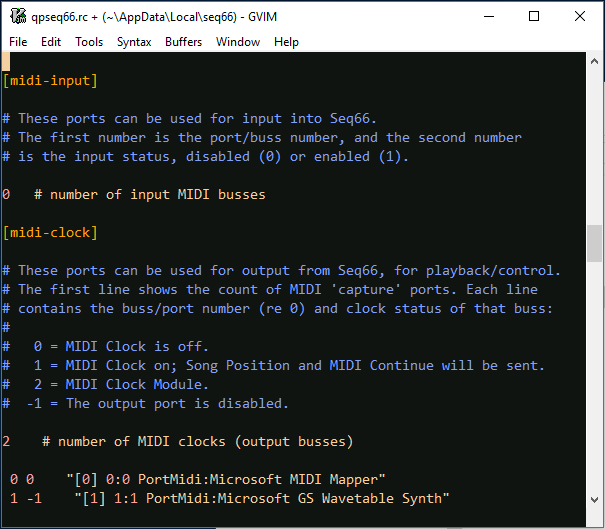
\includegraphics[scale=0.75]{windows/rc-file-post-first-startup.png}
   \caption{'rc' File After Exiting First Startup}
   \label{fig:windows_rc_file_post_first_startup}
\end{figure}

   The \texttt{[midi-input]} section indicates there are no input ports
   (if no MIDI device is connected to the computer).
   The \texttt{[midi-clock]} section indicates there are two output
   ports, and that port 1 is disabled.   So one should be able to
   play a tune to the MIDI mapper and hear it, if output is directed
   to port 0.

   Now run \texttt{qpseq66.exe} again.  No error should appear.
   Go to \textbf{Edit / Preferences / MIDI Clock}.  It might be
   difficult to click on that tab, and we have never figured out why.
   Use \texttt{Alt-C} if necessary.
   It will look like this:

\begin{figure}[H]
   \centering 
   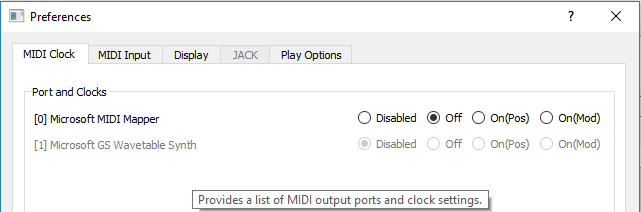
\includegraphics[scale=0.85]{windows/edit-preferences.png}
   \caption{MIDI Output Settings at Second Startup}
   \label{fig:windows_output_settings_second_startup}
\end{figure}

   Next select \textbf{File / Open} and select this sample tune:

   \begin{verbatim}
      C:/Program Files (x86)/Seq66/data/midi/b4uacuse-gm-patchless.midi
   \end{verbatim}

\begin{figure}[H]
   \centering 
   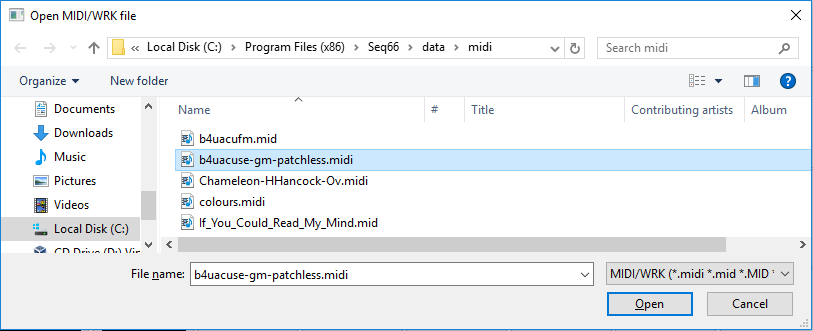
\includegraphics[scale=0.65]{windows/open-installed-midi-file.png}
   \caption{MIDI File Selection}
   \label{fig:windows_open_installed_midi_file}
\end{figure}

   After clicking \textbf{Open}, the following set of patterns is shown.
   Note the two highlighted areas, "Output Selector" and "Song/Live Button".

\begin{figure}[H]
   \centering 
   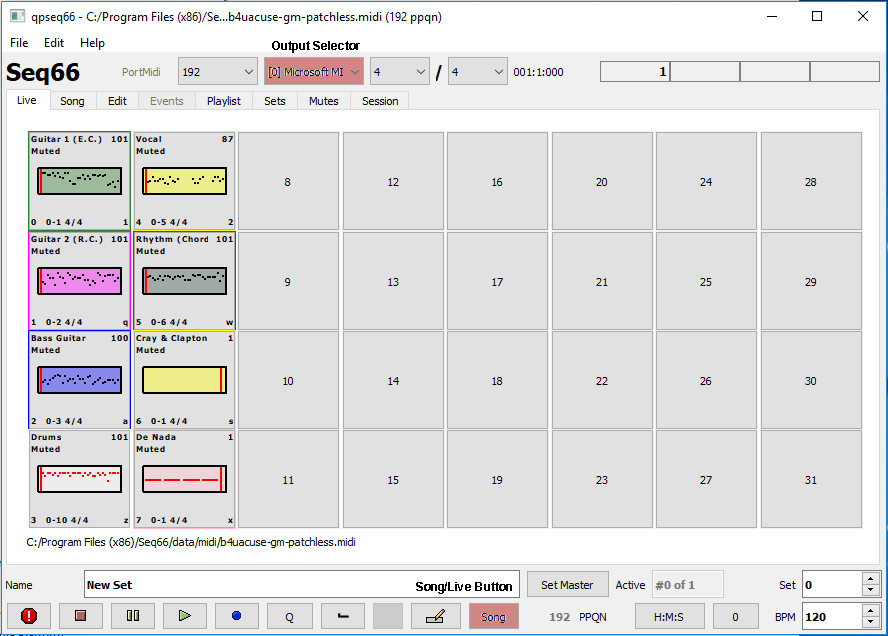
\includegraphics[scale=0.65]{windows/open-midi-file.png}
   \caption{Opened MIDI File}
   \label{fig:windows_open_midi_file}
\end{figure}

   At the top, select port 0 (the MIDI Mapper) from the "Output Selector".
   This \textsl{modifies} the MIDI file so that all MIDI
   output will go to port 0.

   At the bottom, click the "Song/Live Button" until it reads "Song".
   This will access track layouts that turn on all of the patterns.
   These layouts can be seen by selecting the \textbf{Song} tab.

   Now click the play button (green triangle).
   The song should play properly.
   (On our test Windows 10 setup in a virtual machine, playback is ragged,
   but fine on a normal Windows installation on hardware.)

   Overall, the \textsl{Windows} version and the \textsl{Linux} version
   work essentially the same. The \textsl{Linux} version can use the
   \textsl{ALSA} and \textsl{JACK} MIDI engines, while the \textsl{Windows}
   version uses a refactored \textsl{PortMidi} engine that is part of the
   \textsl{Seq66} project.

   The \textsl{PortMidi} engine should also work with \textsl{MacOSX}, but,
   since we don't have a Mac, we haven't been able to build and test
   on that platform.

   Again, for trouble-shooting, also see the installed text file:

   \begin{verbatim}
      C:/Program Files (x86)/Seq66/data/readme.windows
   \end{verbatim}

%-------------------------------------------------------------------------------
% vim: ts=3 sw=3 et ft=tex
%-------------------------------------------------------------------------------
